\chapter{Introduction}
On August 17, 2017, a collision of two  neutron stars produced gravitational waves which were measured by the LIGO and Advanced Virgo detectors, in combination with many other astronomical observatories, marking a new era of advanced multi-messenger observations \cite{ns_2017}, dramatically increasing already very strong interesting in  questions concerning the nature of dense matter in the universe.

Mankind has been interested in the nature of the matter which composes the visible universe, and what are its "constituents" or building blocks. The seminal discovery was made in 1911 by Ernest Rutherford who scattered alpha particles from a gold foil using particles emitted by an alpha source from Marie Curie. His studies led him to conclude that atoms consist of a dense positively charged atomic nucleus surrounded by a dilute electron cloud. Later,  James Chadwick  discovered that the nucleus contained neutral particles -- neutrons  -- in addition to positively charged protons as the basic constituents of nuclear matter. Remarkably, the nucleus itself accounts for 99.9\% of the mass of the atom and only \num{e-12} of the total volume, making it the densest stable form of matter on Earth. 

Without an attractive force between nucleons, the Coulomb force between protons would render the nucleus unstable. It is the strong nuclear force which exerts a large attractive force  between nucleons over a very short range. This strong force is a manifestation of the fundamental interactions between the quarks which constitute each nucleon. Three quarks of two types or \emph{flavors} labeled \emph{up} and \emph{down} with nearly equal masses are needed to form each nucleon. At low energies the internal quark structure of nucleons is less important and nucleons can be thought of as fundamental particles. The strong force between nucleons is attractive only for a small distance of approximately \SIrange{1}{2}{\femto\metre} and becomes very repulsive at even shorter distances, making the nucleus very difficult to compress. It is for this reason that the distance between any pair of nucleons is a near constant value, and therefore the central density value is relatively constant over a wide range of nuclei, from the lightest to the heaviest nuclei \cite{krane}. This density is referred to as the  \emph{saturation density}, since the central density seems to saturate at a common value, namely, $\rho_0 = \SI{1.7e14}{\gram\per\centi\metre\cubed}$ or \num{0.16} nucleons \si{\per\femto\metre\cubed}.  

Due to the nature of the strong force, nuclear matter can be thought of as an in-compressible liquid, in much the same way water exhibits incompressibility. This analogous picture treating nuclei as liquid droplets is remarkably successful at describing the nuclear binding energy $E_{B}$, which is the energy it would take to disassemble a nucleus into its constituents. The Bethe-Weizsacker semi-empirical mass formula \cite{awayforward}, predicts that $E_{B}$ can be expressed as a function of the number of neutrons $N$, protons $Z$, and total nucleons $A = Z + N$:
 
\begin{equation}
E_{B} = a_vA - a_s A^{2/3} - a_c \frac{Z^2}{A^{1/3}} - a_A \frac{(N - Z)^2}{A}
\label{eq:semiEmp}
\end{equation}

Since the strong force makes the inter-nucleon distance approximately constant, the volume the nucleus is related to the total number of nucleons and the volume, $A$. Therefore the first \emph{volume} term $a_VA$ is proportional to $A$. Since the  constituent quarks that make of the nucleons are of nearly equal mass, there is a fundamental symmetry of the strong interaction which the strong interaction between any pair of nuclei is very similar, regardless of the particular flavor of quark composition. This symmetry is called \emph{isospin symmetry}. The term isospin was chosen because this symmetry was similar to the spin symmetry of electrons, which have spin up and down projections but are otherwise indistinguishable, unless in the presence of a symmetry breaking field.  The isospin mathematics are is identical to the spin mathematics describing where nucleons have an isospin of 1/2 and with projections of  +1/2 for protons or -1/2 for neutrons. 

Continuing on with the Bethe-Weizacher formula, we see that there are several correction terms accounting for such effects like the surface, $a_s$, where nucleons near the surface have fewer surrounding neighbors as nucleons inside. Since the volume of the nuclei scales as $A$, radius of the nuclei would scale as $A^{1/3}$. Also there is a correction accounting for the Coulomb force, $a_c$, which is proportional to the radial extent of the nuclei $R^{-1}$; which scales as $A^{1/3}$. The asymmetry term, $a_A$, is related to the difference in energy between adding a neutron or a proton; it is typically referred to as the \emph{symmetry energy}. Although the strong force does not distinguish between protons and neutrons the overall wavefunction is made up of a combination of the spacial, spin, and isospin wavefunctions. Since nucleons are fermions,the total wavefunction must be antisymmetric under particle exchange. Because of this, each spacial and spin state of a nucleon can only be occupied by one neutron and one proton, because there still is isospin asymmetry.  Because of this it is more energetically favorable to form neutron-proton pairs than to become more and more neutron or proton rich. Thus the asymmetry term above is proportional to the factor $\frac{(N - Z)^2}{A}$ which comes directly from Pauli blocking. While Eq.~\ref{eq:semiEmp} describes normal nuclear matter, at saturation density, quite well, a more general description must be made when going to higher or lower densities. 

% This state cannot be occupied by two neutrons or two protons because nucleons are spin 1/2 fermions and the Pauli exclusion principal i.e. "Pauli blocking" only allows one fermion of a specific type (i.e. neutron or proton) per state. The asymmetry term above is proportional to A and the factor $\frac{(N - Z)^2}{A^2}$ comes directly from Pauli blocking. This term is present even when one neglects the nuclear force and approximates the energy of nucleus by that of a Fermi gas. If you add a neutron to a Fermi gas in its ground state, it goes into the lowest energy vacant neutron state. If there is a vacant proton state at lower energy it does not matter because the corresponding neutron state is already filled. This simple consideration accounts for roughly 40 percent of $a_A$. The remaining 60 percent primarily occurs because the nuclear force is most attractive between nucleons in the same state, a configuration that is only allowed if one of the nueleons is a proton and the other is a neutron. In other words, the di-neutron and di-proton form part of the isospin triplet only allowing for the total isospin $T=1$, where as the deuteron (neutron-proton) system may form $T={0,1}$ in the singlet or the triplet, with the singlet being more strongly bound. 

Large macroscopic objects such as neutron stars are composed of mostly pure neutron matter \cite{neutronstar} with a typical size of approximately \SI{11(2)}{\kilo\metre}, though they weigh about 1.5 times the mass of our sun. Such a compact star would normally collapse inward, under its own gravitaitonal force, except for the balancing outward force arising from the strong force which exerts a large outward pressure arising from the symmetry energy at high densities.  The densities reached in a neutron star's interior is a matter of debate. In nucleonic models it is typically 2-4$\rho_o$, but in some quark models for the interior, it can range up to  9$\rho_o$ \cite{neutronstar}. To describe matter at such high densities, the energy density of the system must be described in a more general way than Eq.~\ref{eq:semiEmp}.

%Unlike nuclei, symmetric nuclear matter with equal proton and nucleon densities is not the ground state. This occurs because each proton must be accompanied by an electron in order to locally maintain charge neutrality. This means that the electron density must equal the proton density, which for symmetric matter at normal density puts the electron Fermi energy at xxx MeV.  Because the proton fraction in the interior of a neutron star is typically predicted to be less than 10 percent, the symmetry energy in a neutron star is huge and it gets even larger as one goes into the interior where the density is higher.



Guided by Eq.~\ref{eq:semiEmp}, we can separate the energy density $E$ of a system into two components,

\begin{equation}
E(\rho,\delta) = E(\rho	) + S(\rho)\delta^2,
\label{eq:energyEos}
\end{equation}

where $E(\rho)$ describes the symmetric term (i.e. independent of isospin of the nucleons), and the symmetry energy $S(\rho)$ which depends on the asymmetry of the system, written now in terms of the neutron and proton densities, 

\begin{equation}
\delta = \frac{\rho_n - \rho_p}{\rho}.
\label{eq:asym}
\end{equation}

The Equation of State (EoS) of nuclear matter can be calculated from fundamental thermodynamic relations, 

\begin{equation}
P = \Big(\frac{\delta E}{\delta V}\Big)\vert_{T=0,N}
\label{eq:pressEos}
\end{equation}

for a fixed number of particles $N$ and zero temperature. One can always extend to higher temperatures by adding the typical Boltzman dependence if needed, but here the simplification will suffice. The partial derivative with respects to volume can be rewritten in terms of density:

\begin{equation}
P = -\rho^2 \frac{dE}{d\rho}\vert_{T=0,N}.
\label{eq:densEos}
\end{equation}

The outward pressure generated  by the dense neutron rich matter is related to the derivative -- with respects to density  -- of the symmetry energy \cite{tovEq}. By studying the density dependence of the symmetry energy we can better understand the properties of neutron stars and the dynamics of heavy ion collisions. 

\section{Density Dependence of the Symmetry Energy}

\begin{figure}[!htb]
\centering
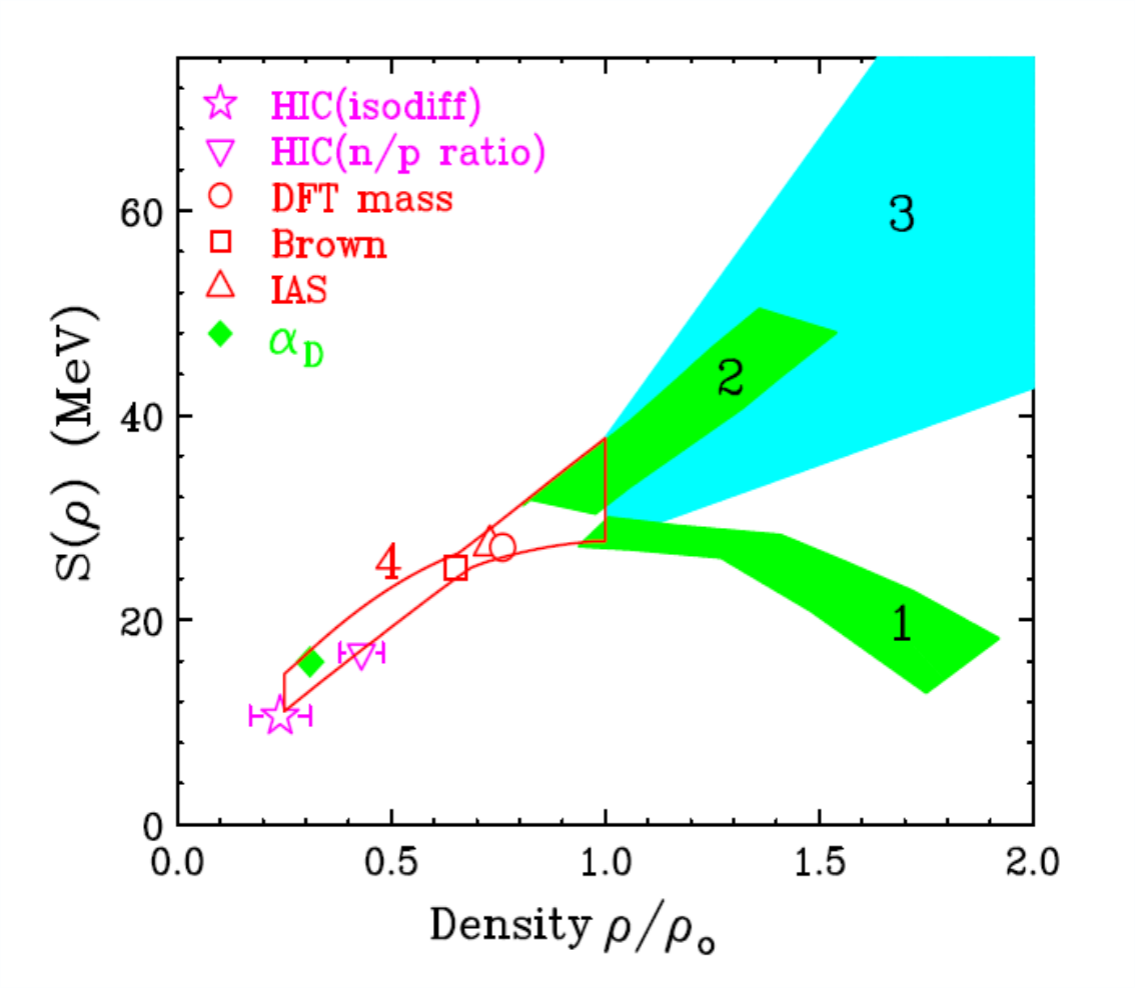
\includegraphics[scale=.3]{densityDep.png}
\caption{Current experimental constraints on the density dependence of the symmetry energy. The measured data points are discussed in the text. The 4 polygonal and shaded regions are constraints from: 1.) pion analysis from Ref. \cite{xia2009,xie2013}, 2.) a separate pion analysis from Ref. \cite{feng2010}, 3.) ASYEOS experiment \cite{russo2011, russo2016, cozma2013} and 4.) isobaric analog states \cite{dan2014} }
\label{fig:symDen}
\end{figure}

In the last couple decades, the symmetric term of Eq.~\ref{eq:energyEos} has been determined for a wide range of densities ranging from $\rho_0 - 4.5\rho_0$ \cite{scienceEos}. In contrast, the symmetry energy has only been accurately constrained for densities at or below $\rho_0$ and only preliminary constraints have been obtained at higher densities. Figure~\ref{fig:symDen} shows the current status of laboratory constrains on on the density dependence of the symmetry energy. The red region labeled 4.) for $\rho < \rho_o$, corresponds to constraints from isobaric analog states \cite{dan2014}. Notice that the symmetry energy is consistent across  a series of independent measurements and observables, but not at higher densities \cite{awayforward}. At higher densities, the two green sections correspond to constriants obtained from total pion yields, and the total pion ratio $\pi^-/\pi^+$, from Au + Au collisions at various beam energies \cite{fopi}. Region 1.) is obtained from analysis performed in References~\cite{xia2009,xie2013} while Region 2.) corresponds to Reference~\cite{feng2010}, giving conflicting results from the same data set. The blue shaded region (labeled 3.) corresponds to constraints obtained through proton and neutron elliptical flow reported in References~\cite{russo2016,cozma2016,cozma2017}. There is still a considerable uncertainty in the symmetry energy at high densities, which are more relevant to neutron stars. It has been the goal of the nuclear EoS community over the last decade to constrain the symmetry energy at these high densities. 




\section{Heavy Ion Collisions}
Besides observing neutron stars directly, heavy-ion collisions (HIC) provide the only way we can probe the density dependence of the symmetry energy in the laboratory setting. When two nuclei collide in a collision, in the very early stages they compress to form a high density region where the nuclei overlap. This momentary density can reach up to $3\rho_0$ depending on the incident beam energy, but only a small volume attains such densities.  HICs also provide the only way we can probe the isospin asymmetry dependence of the nuclear EoS. This is accomplished by using radioactive neutron-rich beams to collide on stable targets. 

The pressure arising from the symmetry energy depends on the curvature of the symmetry energy at a given density as described in Eq.~\ref{eq:densEos}. If the density dependence of the symmetry energy is positive at high densities the symmetry energy would in general force neutrons out of the high density system. If the symmetry energy decreases at high densities, making the derivative  negative, then the symmetry energy term would tend to attract neutrons. The symmetry energy is referred to as \emph{soft} if the second order term in the Taylor expansion -- at saturation density-- is negative, and \emph{stiff} in the case of a curvature that is close to zero or positive. It is the pressure coming from the symmetry energy that is driving the relative dynamics of neutrons and protons, where a stiff symmetry energy expels neutrons from dense matter and vice versa for as soft symmetry energy.

By measuring protons and neutrons, we can see signatures of the symmetry energy in the final spectra of these particles. There are two experimental challenges. First,  measuring neutrons precisely can be quite challenging. The existing technology of neutron time of flight arrays requires long flight paths and large, inefficient detectors. Inevitably, the acceptance is limited by cost and the space required for large neutron wall arrays. Lastly, though the overlap region of the two nuclei temporarily reaches a high density, the nucleons which participated in this region continue to evolve throughout the collision, even into regions of lower densities until they reach their final state. They are continuously interacting with the rest of the nuclear matter, covering a wide range of densities, which dilutes any information about the symmetry energy at at high densities.  




\section{Pion Observable}
\label{sec:pionObs}
Another approach is to find an observable that can be detected with high efficiencies, unlike the neutron, and is more sensitive to the just the high density region. For these reasons pions are a very interesting obserabvle, as they are produced though an intermediate step via production of $\Delta$ resonances. Here the reaction $ NN \leftrightarrow \Delta$ takes place, where nucleon-nucleon collisions form an excited $\Delta$(1232) baryon resonance from one of the nucleons, which then decays shortly thereafter into a pion $\Delta \leftrightarrow \pi N$. The threshold for $\Delta$ resonance production in nucleon-nucleon collisions, with a mass of \SI{1232}{\mega\electronvolt\per\clight\squared}, corresponds to a laboratory beam of \SI{290}{\MeVA} in a fixed target experiment. In large nuclei, the internal motion of the nucleons is substantial and this modifies the production rates. In the Fermi gas model, nucleons are arranged filling up higher energy levels up until they reach the Fermi energy. The associated Fermi velocity can add to the beam velocity and actually be above the threshold condition, even when the beam velocity is below the threshold \cite{fermiEnergy}.


Nuclear collisions are typically calculated via semi-classical theories based on a semi-classical extension of the Boltzmann equation or by semi-classical modifications of molecular dynamics \cite{bertsch}. These theories predict that most of the $\Delta$'s are produced in the early, dense regions of the collision \cite{mingzhang}. Figure~\ref{fig:deltaProduction} shows the average local density in panel (c)  in which $\Delta$'s are produced and the total  number of $\Delta$'s produced in the system (b), as a function of time in the simulation, for Au + Au collisions at \SI{400}{\MeVA}. Panel (a) shows the distribution of density at moment of creation for each $\Delta$. Since the average lifetime of the $\Delta$  is $\tau_{\Delta} = \SI{1.7}{\femto\metre\per\clight}$, the $\Delta$ resonance has very little time to be affected by the medium before decaying into a $\pi$ and nucleon. Thus the outgoing $\pi$ can contains information on the high density region of the collision. 

\begin{figure}[!htb]
\centering
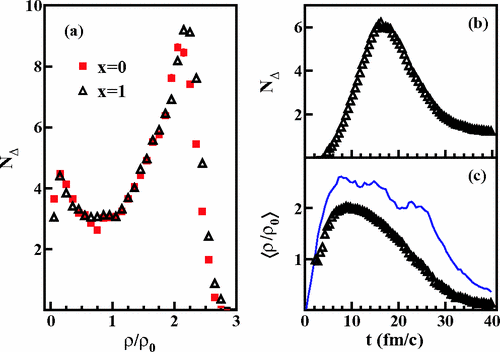
\includegraphics[width=.6\textwidth]{deltaProduction.png}
\caption{Figure taken from \cite{mingzhang} for Au + Au collisions at \SI{400}{\MeVA}. Panel (a) shows the density in the region of the $\Delta$ resonance creation for two different symmetry energies (x=0 soft) and (x=1 stiff). Panel (b) and (c) show the evolution of collision in time steps, where (b) shows the number of deltas in the system as a function of time and (c) shows the mean local baryon density in the region where $\Delta$ resonances are produced. The blue line in (c) represents the average baryon density in the most central region of the collision. This evidence shows that a majority of $\Delta$'s are produced in the high density region of the early collision.}
\label{fig:deltaProduction}
\end{figure}

The branching ratio of the various flavors of $\Delta$'s are given by the Clebsh-Gordon coefficients as shown in Appendix~\ref{appen:deltadecay}. Here we see that in general proton-proton collisions give rise primarily to  $\pi^+$ and neutron-neutron collisions give rise to primarily $\pi^-$. From these branching ratios the charged pion ratio can be described as,

\begin{equation}
\frac{\pi^-}{\pi^+} = \frac{ 5N^2 + ZN }{5Z^2 + ZN}.
\label{eq:deltaModel}
\end{equation}

In this simple $\Delta$ resonance model, $\pi^-/\pi^+ \approx (N/Z)^2$ where $N/Z$ is the neutron-proton ratio of the dense central collision where they are produced. Pions can be reabsorbed into a $\Delta$ resonances after colliding with another nucleon in the backward process of $\Delta \leftrightarrow \pi N$, only to be re-emitted again into a pion. This process generally dilutes the pion sensitivity to the high density region, since with each absorption and re-emission changes the pion dynamics or even the charge of the pion reflecting the neutron-proton asymmetry at the point of creation and re-emission. Total pion absorption, going back into two nucleons, requires a three body process; i.e. the pion collides with a nucleon creating a $\Delta$ resonance, then another nucleon must quickly collide with the resonance to create two nucleons. Since this is a three body process, the total pion absorption (removing them from the system) is a smaller effect than the absorption and re-emission process. Aside from these two effects which degrade the observable, in general the $\pi^-$ are connected with neutrons and the $\pi^+$ production with proton behavior in the high density, early collision; effectively turning the problematic neutron measurement into a charged $\pi^-$ measurement, which is much easier to measure experimentally. It is also directly related to mostly the high density region where the $\Delta$'s are produced.  

\section{Motivation for Thesis}
In an effort to answer the high density behavior of the symmetry energy, we designed a new detector and a set of experiments of Sn + Sn collisions at \SI{270}{\MeVA}. Here we utilized inverse kinematics where the beam is made of a radio-active neutron rich beam, impinging on a stable Sn target. We can probe the isospin asymmetry of the symmetry energy by changing the neutron-proton asymmetry of the incoming beam. Pion production has been studied before in stable beams for beam energies of \SI{400}{\MeVA} and above \cite{fopi}. Yet in these previous experiments, only the total pion yields were published and no pion spectra were published. It was also known that the efficiency analysis of the FOPI detector was particularly difficult especially for low energy pions. In fact the published pion multiplicities are not the measured values but rather extrapolated to low pion energies. We know now that below the cut off cited in \cite{fopi}, approximately 35\% percent of the $\pi^+$ multiplicity and 55\% percent of the $\pi^-$ multiplicity, showing the importance of measuring down to low pion energies. While the pion production increases with the beam energy, this increase is countered by the fact that the effects of the symmetry energy decrease with energy \cite{fopi}. This is because available energy to produce pions is larger and therefore less sensitive to the relatively small symmetry energy.  The goal of this Dissertation was to design and build a high efficiency detector in order to measure pion and light charged particle spectra resulting from HICs. To do this a new Time Projection Chamber (TPC) was made called the SAMURAI pion Reconstruction Ion Tracker (\spirit) TPC.
